\documentclass[twoside]{book}

% Packages required by doxygen
\usepackage{fixltx2e}
\usepackage{calc}
\usepackage{doxygen}
\usepackage[export]{adjustbox} % also loads graphicx
\usepackage{graphicx}
\usepackage[utf8]{inputenc}
\usepackage{makeidx}
\usepackage{multicol}
\usepackage{multirow}
\PassOptionsToPackage{warn}{textcomp}
\usepackage{textcomp}
\usepackage[nointegrals]{wasysym}
\usepackage[table]{xcolor}

% Font selection
\usepackage[T1]{fontenc}
\usepackage[scaled=.90]{helvet}
\usepackage{courier}
\usepackage{amssymb}
\usepackage{sectsty}
\renewcommand{\familydefault}{\sfdefault}
\allsectionsfont{%
  \fontseries{bc}\selectfont%
  \color{darkgray}%
}
\renewcommand{\DoxyLabelFont}{%
  \fontseries{bc}\selectfont%
  \color{darkgray}%
}
\newcommand{\+}{\discretionary{\mbox{\scriptsize$\hookleftarrow$}}{}{}}

% Page & text layout
\usepackage{geometry}
\geometry{%
  a4paper,%
  top=2.5cm,%
  bottom=2.5cm,%
  left=2.5cm,%
  right=2.5cm%
}
\tolerance=750
\hfuzz=15pt
\hbadness=750
\setlength{\emergencystretch}{15pt}
\setlength{\parindent}{0cm}
\setlength{\parskip}{3ex plus 2ex minus 2ex}
\makeatletter
\renewcommand{\paragraph}{%
  \@startsection{paragraph}{4}{0ex}{-1.0ex}{1.0ex}{%
    \normalfont\normalsize\bfseries\SS@parafont%
  }%
}
\renewcommand{\subparagraph}{%
  \@startsection{subparagraph}{5}{0ex}{-1.0ex}{1.0ex}{%
    \normalfont\normalsize\bfseries\SS@subparafont%
  }%
}
\makeatother

% Headers & footers
\usepackage{fancyhdr}
\pagestyle{fancyplain}
\fancyhead[LE]{\fancyplain{}{\bfseries\thepage}}
\fancyhead[CE]{\fancyplain{}{}}
\fancyhead[RE]{\fancyplain{}{\bfseries\leftmark}}
\fancyhead[LO]{\fancyplain{}{\bfseries\rightmark}}
\fancyhead[CO]{\fancyplain{}{}}
\fancyhead[RO]{\fancyplain{}{\bfseries\thepage}}
\fancyfoot[LE]{\fancyplain{}{}}
\fancyfoot[CE]{\fancyplain{}{}}
\fancyfoot[RE]{\fancyplain{}{\bfseries\scriptsize Generated by Doxygen }}
\fancyfoot[LO]{\fancyplain{}{\bfseries\scriptsize Generated by Doxygen }}
\fancyfoot[CO]{\fancyplain{}{}}
\fancyfoot[RO]{\fancyplain{}{}}
\renewcommand{\footrulewidth}{0.4pt}
\renewcommand{\chaptermark}[1]{%
  \markboth{#1}{}%
}
\renewcommand{\sectionmark}[1]{%
  \markright{\thesection\ #1}%
}

% Indices & bibliography
\usepackage{natbib}
\usepackage[titles]{tocloft}
\setcounter{tocdepth}{3}
\setcounter{secnumdepth}{5}
\makeindex

% Hyperlinks (required, but should be loaded last)
\usepackage{ifpdf}
\ifpdf
  \usepackage[pdftex,pagebackref=true]{hyperref}
\else
  \usepackage[ps2pdf,pagebackref=true]{hyperref}
\fi
\hypersetup{%
  colorlinks=true,%
  linkcolor=blue,%
  citecolor=blue,%
  unicode%
}

% Custom commands
\newcommand{\clearemptydoublepage}{%
  \newpage{\pagestyle{empty}\cleardoublepage}%
}

\usepackage{caption}
\captionsetup{labelsep=space,justification=centering,font={bf},singlelinecheck=off,skip=4pt,position=top}

%===== C O N T E N T S =====

\begin{document}

% Titlepage & ToC
\hypersetup{pageanchor=false,
             bookmarksnumbered=true,
             pdfencoding=unicode
            }
\pagenumbering{roman}
\begin{titlepage}
\vspace*{7cm}
\begin{center}%
{\Large My Project }\\
\vspace*{1cm}
{\large Generated by Doxygen 1.8.11}\\
\end{center}
\end{titlepage}
\clearemptydoublepage
\tableofcontents
\clearemptydoublepage
\pagenumbering{arabic}
\hypersetup{pageanchor=true}

%--- Begin generated contents ---
\chapter{Class Index}
\section{Class List}
Here are the classes, structs, unions and interfaces with brief descriptions\+:\begin{DoxyCompactList}
\item\contentsline{section}{\hyperlink{classBall}{Ball} }{\pageref{classBall}}{}
\item\contentsline{section}{\hyperlink{classElement}{Element} }{\pageref{classElement}}{}
\item\contentsline{section}{\hyperlink{classFoodItem}{Food\+Item} }{\pageref{classFoodItem}}{}
\item\contentsline{section}{\hyperlink{classGameBoard}{Game\+Board} }{\pageref{classGameBoard}}{}
\item\contentsline{section}{\hyperlink{classPlayer}{Player} }{\pageref{classPlayer}}{}
\item\contentsline{section}{\hyperlink{classStat}{Stat} }{\pageref{classStat}}{}
\item\contentsline{section}{\hyperlink{structUpdateElementData}{Update\+Element\+Data} }{\pageref{structUpdateElementData}}{}
\item\contentsline{section}{\hyperlink{classWebServer}{Web\+Server} }{\pageref{classWebServer}}{}
\end{DoxyCompactList}

\chapter{File Index}
\section{File List}
Here is a list of all documented files with brief descriptions\+:\begin{DoxyCompactList}
\item\contentsline{section}{{\bfseries ball.\+hpp} }{\pageref{ball_8hpp}}{}
\item\contentsline{section}{{\bfseries element.\+hpp} }{\pageref{element_8hpp}}{}
\item\contentsline{section}{{\bfseries food\+Item.\+hpp} }{\pageref{foodItem_8hpp}}{}
\item\contentsline{section}{{\bfseries game\+Board.\+hpp} }{\pageref{gameBoard_8hpp}}{}
\item\contentsline{section}{\hyperlink{main_8cpp}{main.\+cpp} }{\pageref{main_8cpp}}{}
\item\contentsline{section}{{\bfseries player.\+hpp} }{\pageref{player_8hpp}}{}
\item\contentsline{section}{{\bfseries stat.\+hpp} }{\pageref{stat_8hpp}}{}
\item\contentsline{section}{{\bfseries webserver.\+hpp} }{\pageref{webserver_8hpp}}{}
\end{DoxyCompactList}

\chapter{Class Documentation}
\hypertarget{classBall}{}\section{Ball Class Reference}
\label{classBall}\index{Ball@{Ball}}


Inheritance diagram for Ball\+:
\nopagebreak
\begin{figure}[H]
\begin{center}
\leavevmode
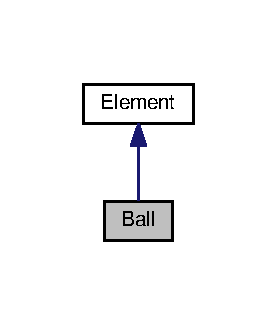
\includegraphics[width=133pt]{classBall__inherit__graph}
\end{center}
\end{figure}


Collaboration diagram for Ball\+:
\nopagebreak
\begin{figure}[H]
\begin{center}
\leavevmode
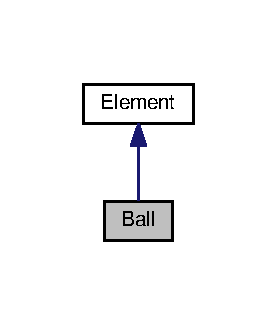
\includegraphics[width=133pt]{classBall__coll__graph}
\end{center}
\end{figure}
\subsection*{Public Member Functions}
\begin{DoxyCompactItemize}
\item 
virtual void {\bfseries notify} ()\hypertarget{classBall_aac709d26ebeb71a87af845dc8c2316a2}{}\label{classBall_aac709d26ebeb71a87af845dc8c2316a2}

\item 
void {\bfseries increase\+Mass} (int add\+\_\+mass)\hypertarget{classBall_a39e9307ae41f0b651315c5d0dbb30b73}{}\label{classBall_a39e9307ae41f0b651315c5d0dbb30b73}

\end{DoxyCompactItemize}


The documentation for this class was generated from the following file\+:\begin{DoxyCompactItemize}
\item 
ball.\+hpp\end{DoxyCompactItemize}

\hypertarget{classFood}{}\section{Food Class Reference}
\label{classFood}\index{Food@{Food}}
\subsection*{Public Member Functions}
\begin{DoxyCompactItemize}
\item 
\hyperlink{classFood_aec4053e5cb44b46370d4e2e5b23745f3}{constructor} (id, x, y, color)
\begin{DoxyCompactList}\small\item\em \hyperlink{classFood}{Food} constructor. \end{DoxyCompactList}\item 
\hyperlink{classFood_ae25f8cd59957446522973ebf902ad6c3}{show} ()
\begin{DoxyCompactList}\small\item\em Display food on screen. \end{DoxyCompactList}\end{DoxyCompactItemize}


\subsection{Member Function Documentation}
\index{Food@{Food}!constructor@{constructor}}
\index{constructor@{constructor}!Food@{Food}}
\subsubsection[{\texorpdfstring{constructor(id, x, y, color)}{constructor(id, x, y, color)}}]{\setlength{\rightskip}{0pt plus 5cm}Food\+::constructor (
\begin{DoxyParamCaption}
\item[{}]{id, }
\item[{}]{x, }
\item[{}]{y, }
\item[{}]{color}
\end{DoxyParamCaption}
)\hspace{0.3cm}{\ttfamily [inline]}}\hypertarget{classFood_aec4053e5cb44b46370d4e2e5b23745f3}{}\label{classFood_aec4053e5cb44b46370d4e2e5b23745f3}


\hyperlink{classFood}{Food} constructor. 

\index{Food@{Food}!show@{show}}
\index{show@{show}!Food@{Food}}
\subsubsection[{\texorpdfstring{show()}{show()}}]{\setlength{\rightskip}{0pt plus 5cm}Food\+::show (
\begin{DoxyParamCaption}
{}
\end{DoxyParamCaption}
)\hspace{0.3cm}{\ttfamily [inline]}}\hypertarget{classFood_ae25f8cd59957446522973ebf902ad6c3}{}\label{classFood_ae25f8cd59957446522973ebf902ad6c3}


Display food on screen. 



The documentation for this class was generated from the following file\+:\begin{DoxyCompactItemize}
\item 
\hyperlink{food_8js}{food.\+js}\end{DoxyCompactItemize}

\hypertarget{classPlayer}{}\section{Player Class Reference}
\label{classPlayer}\index{Player@{Player}}
\subsection*{Public Member Functions}
\begin{DoxyCompactItemize}
\item 
\hyperlink{classPlayer_ab5c49386411a5e649c8a6328d5a510f8}{constructor} (id, x, y, r, color, name)
\begin{DoxyCompactList}\small\item\em \hyperlink{classPlayer}{Player} constructor. \end{DoxyCompactList}\item 
\hyperlink{classPlayer_a619a6d875382df23fcd0cf423e233b3a}{show} ()
\begin{DoxyCompactList}\small\item\em Display player on screen. \end{DoxyCompactList}\end{DoxyCompactItemize}


\subsection{Member Function Documentation}
\index{Player@{Player}!constructor@{constructor}}
\index{constructor@{constructor}!Player@{Player}}
\subsubsection[{\texorpdfstring{constructor(id, x, y, r, color, name)}{constructor(id, x, y, r, color, name)}}]{\setlength{\rightskip}{0pt plus 5cm}Player\+::constructor (
\begin{DoxyParamCaption}
\item[{}]{id, }
\item[{}]{x, }
\item[{}]{y, }
\item[{}]{r, }
\item[{}]{color, }
\item[{}]{name}
\end{DoxyParamCaption}
)\hspace{0.3cm}{\ttfamily [inline]}}\hypertarget{classPlayer_ab5c49386411a5e649c8a6328d5a510f8}{}\label{classPlayer_ab5c49386411a5e649c8a6328d5a510f8}


\hyperlink{classPlayer}{Player} constructor. 

\index{Player@{Player}!show@{show}}
\index{show@{show}!Player@{Player}}
\subsubsection[{\texorpdfstring{show()}{show()}}]{\setlength{\rightskip}{0pt plus 5cm}Player\+::show (
\begin{DoxyParamCaption}
{}
\end{DoxyParamCaption}
)\hspace{0.3cm}{\ttfamily [inline]}}\hypertarget{classPlayer_a619a6d875382df23fcd0cf423e233b3a}{}\label{classPlayer_a619a6d875382df23fcd0cf423e233b3a}


Display player on screen. 



The documentation for this class was generated from the following file\+:\begin{DoxyCompactItemize}
\item 
\hyperlink{player_8js}{player.\+js}\end{DoxyCompactItemize}

\chapter{File Documentation}
\hypertarget{app_8js}{}\section{app.\+js File Reference}
\label{app_8js}\index{app.\+js@{app.\+js}}
\subsection*{Functions}
\begin{DoxyCompactItemize}
\item 
window \hyperlink{app_8js_a6c854fdf43b195a051418c43e4d6440b}{add\+Event\+Listener} (\textquotesingle{}resize\textquotesingle{}, \hyperlink{app_8js_a9f60d5caf0aa8d90f9b74c79623657a1}{resize\+Canvas}, false)
\item 
\hyperlink{app_8js_a9f60d5caf0aa8d90f9b74c79623657a1}{resize\+Canvas} ()
\begin{DoxyCompactList}\small\item\em Resize canvas handle. \end{DoxyCompactList}\item 
function \hyperlink{app_8js_a95be355e63bd2ce5d1d244b331782be8}{get\+Random\+Color} ()
\begin{DoxyCompactList}\small\item\em Returns random color. \end{DoxyCompactList}\item 
function \hyperlink{app_8js_a7f7e0f25b5ea7ad26a201878d16df270}{is\+Nick\+Valid} ()
\begin{DoxyCompactList}\small\item\em Validates nickname. \end{DoxyCompactList}\item 
function \hyperlink{app_8js_a43d52d4fb2afd79df202b46772f2ad13}{on\+Error} (evt)
\begin{DoxyCompactList}\small\item\em Error handle. \end{DoxyCompactList}\item 
function \hyperlink{app_8js_aceb05684e085976addee08f3ef78165c}{get\+Mouse\+Pos} (\hyperlink{app_8js_a1c82fafbefefac03f47e6f1a3cad5b73}{canvas}, evt)
\begin{DoxyCompactList}\small\item\em Mouse handle. \end{DoxyCompactList}\item 
function \hyperlink{app_8js_ab297afd9d563d4114a23680863e53d80}{update} ()
\begin{DoxyCompactList}\small\item\em Display update (Animation) \end{DoxyCompactList}\item 
function \hyperlink{app_8js_a3de7939030ae291bccf65f65cb133670}{calculate\+Fixed\+Pos} ()
\begin{DoxyCompactList}\small\item\em Calculate object\textquotesingle{}s fx,fy distance from player\textquotesingle{}s center of screen. \end{DoxyCompactList}\item 
function \hyperlink{app_8js_a32c8954b3abac7767adc4cbbb6b267d2}{game\+Over} ()
\begin{DoxyCompactList}\small\item\em Game\+Over handle. \end{DoxyCompactList}\item 
function \hyperlink{app_8js_ab310d9a3a26705f282a24c69326ec4a1}{start\+Game} ()
\begin{DoxyCompactList}\small\item\em Start\+Game handle. \end{DoxyCompactList}\end{DoxyCompactItemize}
\subsection*{Variables}
\begin{DoxyCompactItemize}
\item 
var \hyperlink{app_8js_a1c82fafbefefac03f47e6f1a3cad5b73}{canvas} = document.\+get\+Element\+By\+Id(\textquotesingle{}cvs\textquotesingle{})
\item 
var \hyperlink{app_8js_a052064742b5acc950df6b3c78d4ecd65}{context} = canvas.\+get\+Context(\textquotesingle{}2d\textquotesingle{})
\item 
var \hyperlink{app_8js_aaf620ad7a23011f857f80e457b23d609}{raf}
\item 
var \hyperlink{app_8js_a5512c9740e5f6440179f46ce633b28f0}{balls} = \mbox{[}$\,$\mbox{]}
\item 
var \hyperlink{app_8js_adae9690bde328f9ed2e75254eec08cb3}{foods} = \mbox{[}$\,$\mbox{]}
\item 
var \hyperlink{app_8js_ac1e8507dd4816b1d5fd78a420119975e}{mouse\+Pos}
\item 
var \hyperlink{app_8js_af4a3cb26e92251a48cee128ae9778a75}{player} = 0
\item 
var \hyperlink{app_8js_aa267fb6b258db6dbd04a6b878c9e6898}{scl} = 1
\item 
var \hyperlink{app_8js_a893d4967ef1870c2617590d4509659f6}{board\+Margin} = 0
\item 
var \hyperlink{app_8js_ae50d618b57a465c2838ed97c28ad4127}{game\+BoardX}
\item 
var \hyperlink{app_8js_a7d046795e7d6fae389363f32afaa22bf}{game\+BoardY}
\item 
var \hyperlink{app_8js_a8f2b7ad1a2948d6017f40e5e1e992ab5}{deltaX}
\item 
var \hyperlink{app_8js_aa8908a60e69cb0bab3e527a130edde55}{deltaY}
\item 
var \hyperlink{app_8js_a2fb56143c564f962700db007b34eeab6}{game\+Start} = false
\item 
var \hyperlink{app_8js_a421b77753876b4010bdb1d276e068867}{game\+Died} = false
\item 
var \hyperlink{app_8js_a570cad7abdfa4176776d7e9bff76ed63}{player\+Set} = false
\item 
var \hyperlink{app_8js_abe333e9c5c7687e5729ae6fae360c032}{death\+Stats} = \mbox{[}0, 0, 0\mbox{]}
\end{DoxyCompactItemize}


\subsection{Detailed Description}
\begin{DoxyAuthor}{Author}
Wojciech Przybysz, Kajetan Spionek Main application file 
\end{DoxyAuthor}


\subsection{Function Documentation}
\index{app.\+js@{app.\+js}!add\+Event\+Listener@{add\+Event\+Listener}}
\index{add\+Event\+Listener@{add\+Event\+Listener}!app.\+js@{app.\+js}}
\subsubsection[{\texorpdfstring{add\+Event\+Listener(\textquotesingle{}resize\textquotesingle{}, resize\+Canvas, false)}{addEventListener('resize', resizeCanvas, false)}}]{\setlength{\rightskip}{0pt plus 5cm}window add\+Event\+Listener (
\begin{DoxyParamCaption}
\item[{\textquotesingle{}resize\textquotesingle{}}]{, }
\item[{{\bf resize\+Canvas}}]{, }
\item[{false}]{}
\end{DoxyParamCaption}
)}\hypertarget{app_8js_a6c854fdf43b195a051418c43e4d6440b}{}\label{app_8js_a6c854fdf43b195a051418c43e4d6440b}
\index{app.\+js@{app.\+js}!calculate\+Fixed\+Pos@{calculate\+Fixed\+Pos}}
\index{calculate\+Fixed\+Pos@{calculate\+Fixed\+Pos}!app.\+js@{app.\+js}}
\subsubsection[{\texorpdfstring{calculate\+Fixed\+Pos()}{calculateFixedPos()}}]{\setlength{\rightskip}{0pt plus 5cm}function calculate\+Fixed\+Pos (
\begin{DoxyParamCaption}
{}
\end{DoxyParamCaption}
)}\hypertarget{app_8js_a3de7939030ae291bccf65f65cb133670}{}\label{app_8js_a3de7939030ae291bccf65f65cb133670}


Calculate object\textquotesingle{}s fx,fy distance from player\textquotesingle{}s center of screen. 

\index{app.\+js@{app.\+js}!game\+Over@{game\+Over}}
\index{game\+Over@{game\+Over}!app.\+js@{app.\+js}}
\subsubsection[{\texorpdfstring{game\+Over()}{gameOver()}}]{\setlength{\rightskip}{0pt plus 5cm}function game\+Over (
\begin{DoxyParamCaption}
{}
\end{DoxyParamCaption}
)}\hypertarget{app_8js_a32c8954b3abac7767adc4cbbb6b267d2}{}\label{app_8js_a32c8954b3abac7767adc4cbbb6b267d2}


Game\+Over handle. 

\index{app.\+js@{app.\+js}!get\+Mouse\+Pos@{get\+Mouse\+Pos}}
\index{get\+Mouse\+Pos@{get\+Mouse\+Pos}!app.\+js@{app.\+js}}
\subsubsection[{\texorpdfstring{get\+Mouse\+Pos(canvas, evt)}{getMousePos(canvas, evt)}}]{\setlength{\rightskip}{0pt plus 5cm}function get\+Mouse\+Pos (
\begin{DoxyParamCaption}
\item[{}]{canvas, }
\item[{}]{evt}
\end{DoxyParamCaption}
)}\hypertarget{app_8js_aceb05684e085976addee08f3ef78165c}{}\label{app_8js_aceb05684e085976addee08f3ef78165c}


Mouse handle. 

\index{app.\+js@{app.\+js}!get\+Random\+Color@{get\+Random\+Color}}
\index{get\+Random\+Color@{get\+Random\+Color}!app.\+js@{app.\+js}}
\subsubsection[{\texorpdfstring{get\+Random\+Color()}{getRandomColor()}}]{\setlength{\rightskip}{0pt plus 5cm}function get\+Random\+Color (
\begin{DoxyParamCaption}
{}
\end{DoxyParamCaption}
)}\hypertarget{app_8js_a95be355e63bd2ce5d1d244b331782be8}{}\label{app_8js_a95be355e63bd2ce5d1d244b331782be8}


Returns random color. 

\index{app.\+js@{app.\+js}!is\+Nick\+Valid@{is\+Nick\+Valid}}
\index{is\+Nick\+Valid@{is\+Nick\+Valid}!app.\+js@{app.\+js}}
\subsubsection[{\texorpdfstring{is\+Nick\+Valid()}{isNickValid()}}]{\setlength{\rightskip}{0pt plus 5cm}function is\+Nick\+Valid (
\begin{DoxyParamCaption}
{}
\end{DoxyParamCaption}
)}\hypertarget{app_8js_a7f7e0f25b5ea7ad26a201878d16df270}{}\label{app_8js_a7f7e0f25b5ea7ad26a201878d16df270}


Validates nickname. 

\index{app.\+js@{app.\+js}!on\+Error@{on\+Error}}
\index{on\+Error@{on\+Error}!app.\+js@{app.\+js}}
\subsubsection[{\texorpdfstring{on\+Error(evt)}{onError(evt)}}]{\setlength{\rightskip}{0pt plus 5cm}function on\+Error (
\begin{DoxyParamCaption}
\item[{}]{evt}
\end{DoxyParamCaption}
)}\hypertarget{app_8js_a43d52d4fb2afd79df202b46772f2ad13}{}\label{app_8js_a43d52d4fb2afd79df202b46772f2ad13}


Error handle. 

\index{app.\+js@{app.\+js}!resize\+Canvas@{resize\+Canvas}}
\index{resize\+Canvas@{resize\+Canvas}!app.\+js@{app.\+js}}
\subsubsection[{\texorpdfstring{resize\+Canvas()}{resizeCanvas()}}]{\setlength{\rightskip}{0pt plus 5cm}function resize\+Canvas (
\begin{DoxyParamCaption}
{}
\end{DoxyParamCaption}
)}\hypertarget{app_8js_a9f60d5caf0aa8d90f9b74c79623657a1}{}\label{app_8js_a9f60d5caf0aa8d90f9b74c79623657a1}


Resize canvas handle. 

\index{app.\+js@{app.\+js}!start\+Game@{start\+Game}}
\index{start\+Game@{start\+Game}!app.\+js@{app.\+js}}
\subsubsection[{\texorpdfstring{start\+Game()}{startGame()}}]{\setlength{\rightskip}{0pt plus 5cm}function start\+Game (
\begin{DoxyParamCaption}
{}
\end{DoxyParamCaption}
)}\hypertarget{app_8js_ab310d9a3a26705f282a24c69326ec4a1}{}\label{app_8js_ab310d9a3a26705f282a24c69326ec4a1}


Start\+Game handle. 

\index{app.\+js@{app.\+js}!update@{update}}
\index{update@{update}!app.\+js@{app.\+js}}
\subsubsection[{\texorpdfstring{update()}{update()}}]{\setlength{\rightskip}{0pt plus 5cm}function update (
\begin{DoxyParamCaption}
{}
\end{DoxyParamCaption}
)}\hypertarget{app_8js_ab297afd9d563d4114a23680863e53d80}{}\label{app_8js_ab297afd9d563d4114a23680863e53d80}


Display update (Animation) 



\subsection{Variable Documentation}
\index{app.\+js@{app.\+js}!balls@{balls}}
\index{balls@{balls}!app.\+js@{app.\+js}}
\subsubsection[{\texorpdfstring{balls}{balls}}]{\setlength{\rightskip}{0pt plus 5cm}var balls = \mbox{[}$\,$\mbox{]}}\hypertarget{app_8js_a5512c9740e5f6440179f46ce633b28f0}{}\label{app_8js_a5512c9740e5f6440179f46ce633b28f0}
\index{app.\+js@{app.\+js}!board\+Margin@{board\+Margin}}
\index{board\+Margin@{board\+Margin}!app.\+js@{app.\+js}}
\subsubsection[{\texorpdfstring{board\+Margin}{boardMargin}}]{\setlength{\rightskip}{0pt plus 5cm}var board\+Margin = 0}\hypertarget{app_8js_a893d4967ef1870c2617590d4509659f6}{}\label{app_8js_a893d4967ef1870c2617590d4509659f6}
\index{app.\+js@{app.\+js}!canvas@{canvas}}
\index{canvas@{canvas}!app.\+js@{app.\+js}}
\subsubsection[{\texorpdfstring{canvas}{canvas}}]{\setlength{\rightskip}{0pt plus 5cm}var canvas = document.\+get\+Element\+By\+Id(\textquotesingle{}cvs\textquotesingle{})}\hypertarget{app_8js_a1c82fafbefefac03f47e6f1a3cad5b73}{}\label{app_8js_a1c82fafbefefac03f47e6f1a3cad5b73}
\index{app.\+js@{app.\+js}!context@{context}}
\index{context@{context}!app.\+js@{app.\+js}}
\subsubsection[{\texorpdfstring{context}{context}}]{\setlength{\rightskip}{0pt plus 5cm}var context = canvas.\+get\+Context(\textquotesingle{}2d\textquotesingle{})}\hypertarget{app_8js_a052064742b5acc950df6b3c78d4ecd65}{}\label{app_8js_a052064742b5acc950df6b3c78d4ecd65}
\index{app.\+js@{app.\+js}!death\+Stats@{death\+Stats}}
\index{death\+Stats@{death\+Stats}!app.\+js@{app.\+js}}
\subsubsection[{\texorpdfstring{death\+Stats}{deathStats}}]{\setlength{\rightskip}{0pt plus 5cm}var death\+Stats = \mbox{[}0, 0, 0\mbox{]}}\hypertarget{app_8js_abe333e9c5c7687e5729ae6fae360c032}{}\label{app_8js_abe333e9c5c7687e5729ae6fae360c032}
\index{app.\+js@{app.\+js}!deltaX@{deltaX}}
\index{deltaX@{deltaX}!app.\+js@{app.\+js}}
\subsubsection[{\texorpdfstring{deltaX}{deltaX}}]{\setlength{\rightskip}{0pt plus 5cm}var deltaX}\hypertarget{app_8js_a8f2b7ad1a2948d6017f40e5e1e992ab5}{}\label{app_8js_a8f2b7ad1a2948d6017f40e5e1e992ab5}
\index{app.\+js@{app.\+js}!deltaY@{deltaY}}
\index{deltaY@{deltaY}!app.\+js@{app.\+js}}
\subsubsection[{\texorpdfstring{deltaY}{deltaY}}]{\setlength{\rightskip}{0pt plus 5cm}var deltaY}\hypertarget{app_8js_aa8908a60e69cb0bab3e527a130edde55}{}\label{app_8js_aa8908a60e69cb0bab3e527a130edde55}
\index{app.\+js@{app.\+js}!foods@{foods}}
\index{foods@{foods}!app.\+js@{app.\+js}}
\subsubsection[{\texorpdfstring{foods}{foods}}]{\setlength{\rightskip}{0pt plus 5cm}var foods = \mbox{[}$\,$\mbox{]}}\hypertarget{app_8js_adae9690bde328f9ed2e75254eec08cb3}{}\label{app_8js_adae9690bde328f9ed2e75254eec08cb3}
\index{app.\+js@{app.\+js}!game\+BoardX@{game\+BoardX}}
\index{game\+BoardX@{game\+BoardX}!app.\+js@{app.\+js}}
\subsubsection[{\texorpdfstring{game\+BoardX}{gameBoardX}}]{\setlength{\rightskip}{0pt plus 5cm}var game\+BoardX}\hypertarget{app_8js_ae50d618b57a465c2838ed97c28ad4127}{}\label{app_8js_ae50d618b57a465c2838ed97c28ad4127}
\index{app.\+js@{app.\+js}!game\+BoardY@{game\+BoardY}}
\index{game\+BoardY@{game\+BoardY}!app.\+js@{app.\+js}}
\subsubsection[{\texorpdfstring{game\+BoardY}{gameBoardY}}]{\setlength{\rightskip}{0pt plus 5cm}var game\+BoardY}\hypertarget{app_8js_a7d046795e7d6fae389363f32afaa22bf}{}\label{app_8js_a7d046795e7d6fae389363f32afaa22bf}
\index{app.\+js@{app.\+js}!game\+Died@{game\+Died}}
\index{game\+Died@{game\+Died}!app.\+js@{app.\+js}}
\subsubsection[{\texorpdfstring{game\+Died}{gameDied}}]{\setlength{\rightskip}{0pt plus 5cm}var game\+Died = false}\hypertarget{app_8js_a421b77753876b4010bdb1d276e068867}{}\label{app_8js_a421b77753876b4010bdb1d276e068867}
\index{app.\+js@{app.\+js}!game\+Start@{game\+Start}}
\index{game\+Start@{game\+Start}!app.\+js@{app.\+js}}
\subsubsection[{\texorpdfstring{game\+Start}{gameStart}}]{\setlength{\rightskip}{0pt plus 5cm}var game\+Start = false}\hypertarget{app_8js_a2fb56143c564f962700db007b34eeab6}{}\label{app_8js_a2fb56143c564f962700db007b34eeab6}
\index{app.\+js@{app.\+js}!mouse\+Pos@{mouse\+Pos}}
\index{mouse\+Pos@{mouse\+Pos}!app.\+js@{app.\+js}}
\subsubsection[{\texorpdfstring{mouse\+Pos}{mousePos}}]{\setlength{\rightskip}{0pt plus 5cm}var mouse\+Pos}\hypertarget{app_8js_ac1e8507dd4816b1d5fd78a420119975e}{}\label{app_8js_ac1e8507dd4816b1d5fd78a420119975e}
\index{app.\+js@{app.\+js}!player@{player}}
\index{player@{player}!app.\+js@{app.\+js}}
\subsubsection[{\texorpdfstring{player}{player}}]{\setlength{\rightskip}{0pt plus 5cm}var player = 0}\hypertarget{app_8js_af4a3cb26e92251a48cee128ae9778a75}{}\label{app_8js_af4a3cb26e92251a48cee128ae9778a75}
\index{app.\+js@{app.\+js}!player\+Set@{player\+Set}}
\index{player\+Set@{player\+Set}!app.\+js@{app.\+js}}
\subsubsection[{\texorpdfstring{player\+Set}{playerSet}}]{\setlength{\rightskip}{0pt plus 5cm}var player\+Set = false}\hypertarget{app_8js_a570cad7abdfa4176776d7e9bff76ed63}{}\label{app_8js_a570cad7abdfa4176776d7e9bff76ed63}
\index{app.\+js@{app.\+js}!raf@{raf}}
\index{raf@{raf}!app.\+js@{app.\+js}}
\subsubsection[{\texorpdfstring{raf}{raf}}]{\setlength{\rightskip}{0pt plus 5cm}var raf}\hypertarget{app_8js_aaf620ad7a23011f857f80e457b23d609}{}\label{app_8js_aaf620ad7a23011f857f80e457b23d609}
\index{app.\+js@{app.\+js}!scl@{scl}}
\index{scl@{scl}!app.\+js@{app.\+js}}
\subsubsection[{\texorpdfstring{scl}{scl}}]{\setlength{\rightskip}{0pt plus 5cm}var scl = 1}\hypertarget{app_8js_aa267fb6b258db6dbd04a6b878c9e6898}{}\label{app_8js_aa267fb6b258db6dbd04a6b878c9e6898}

\hypertarget{ball_8js}{}\section{ball.\+js File Reference}
\label{ball_8js}\index{ball.\+js@{ball.\+js}}
\subsection*{Classes}
\begin{DoxyCompactItemize}
\item 
class \hyperlink{classBall}{Ball}
\end{DoxyCompactItemize}


\subsection{Detailed Description}
\begin{DoxyAuthor}{Author}
Wojciech Przybysz, Kajetan Spionek Implementation of ball class 
\end{DoxyAuthor}

\hypertarget{canvas_8js}{}\section{canvas.\+js File Reference}
\label{canvas_8js}\index{canvas.\+js@{canvas.\+js}}
\subsection*{Functions}
\begin{DoxyCompactItemize}
\item 
\hyperlink{app_8js_a1c82fafbefefac03f47e6f1a3cad5b73}{canvas} \hyperlink{canvas_8js_aaf6560b22d7358542ce9da3e6c487cf6}{add\+Event\+Listener} (\textquotesingle{}mousemove\textquotesingle{}, function(evt)\{\hyperlink{app_8js_ac1e8507dd4816b1d5fd78a420119975e}{mouse\+Pos}=\hyperlink{app_8js_aceb05684e085976addee08f3ef78165c}{get\+Mouse\+Pos}(\hyperlink{app_8js_a1c82fafbefefac03f47e6f1a3cad5b73}{canvas}, evt);\})
\item 
function \hyperlink{canvas_8js_adb3fc5e797db510a62c23541162f302a}{draw\+Circle} (x\+\_\+center, y\+\_\+center, radius, color)
\begin{DoxyCompactList}\small\item\em Draws circle on x,y position. \end{DoxyCompactList}\item 
function \hyperlink{canvas_8js_a71c2eb1c63790a302cd3cc6dd3880bd1}{draw\+Circle\+Fx} (fx\+\_\+center, fy\+\_\+center, radius, color)
\begin{DoxyCompactList}\small\item\em Draws circle within fx,fy distance from center of player\textquotesingle{}s screen. \end{DoxyCompactList}\item 
function \hyperlink{canvas_8js_a8ec1f5e4b3953abf0dc7243ae720d4b2}{re\+Draw\+Grid} ()
\begin{DoxyCompactList}\small\item\em Redraws grid. \end{DoxyCompactList}\item 
function \hyperlink{canvas_8js_afa70c0c095a4753036e0456c463818e6}{re\+Draw\+Canvas} ()
\begin{DoxyCompactList}\small\item\em Draws objects on map (player, balls and food) \end{DoxyCompactList}\item 
function \hyperlink{canvas_8js_adba1fd186c14805ce7552d539d51eac3}{death\+Screen} ()
\begin{DoxyCompactList}\small\item\em Displays death screen on canvas. \end{DoxyCompactList}\end{DoxyCompactItemize}
\subsection*{Variables}
\begin{DoxyCompactItemize}
\item 
window \hyperlink{canvas_8js_abca23acbc1d398418271025c99640f01}{request\+Anim\+Frame}
\item 
window \hyperlink{canvas_8js_a4b4effc24650c2ef5245e327686ca601}{cancel\+Anim\+Frame}
\end{DoxyCompactItemize}


\subsection{Function Documentation}
\index{canvas.\+js@{canvas.\+js}!add\+Event\+Listener@{add\+Event\+Listener}}
\index{add\+Event\+Listener@{add\+Event\+Listener}!canvas.\+js@{canvas.\+js}}
\subsubsection[{\texorpdfstring{add\+Event\+Listener(\textquotesingle{}mousemove\textquotesingle{}, function(evt)\lcurly{}mouse\+Pos=get\+Mouse\+Pos(canvas, evt);\rcurly{})}{addEventListener('mousemove', function(evt)\{mousePos=getMousePos(canvas, evt);\})}}]{\setlength{\rightskip}{0pt plus 5cm}{\bf canvas} add\+Event\+Listener (
\begin{DoxyParamCaption}
\item[{\textquotesingle{}mousemove\textquotesingle{}}]{, }
\item[{function(evt)\{{\bf mouse\+Pos}={\bf get\+Mouse\+Pos}({\bf canvas}, evt);\}}]{}
\end{DoxyParamCaption}
)}\hypertarget{canvas_8js_aaf6560b22d7358542ce9da3e6c487cf6}{}\label{canvas_8js_aaf6560b22d7358542ce9da3e6c487cf6}
\index{canvas.\+js@{canvas.\+js}!death\+Screen@{death\+Screen}}
\index{death\+Screen@{death\+Screen}!canvas.\+js@{canvas.\+js}}
\subsubsection[{\texorpdfstring{death\+Screen()}{deathScreen()}}]{\setlength{\rightskip}{0pt plus 5cm}function death\+Screen (
\begin{DoxyParamCaption}
{}
\end{DoxyParamCaption}
)}\hypertarget{canvas_8js_adba1fd186c14805ce7552d539d51eac3}{}\label{canvas_8js_adba1fd186c14805ce7552d539d51eac3}


Displays death screen on canvas. 

\index{canvas.\+js@{canvas.\+js}!draw\+Circle@{draw\+Circle}}
\index{draw\+Circle@{draw\+Circle}!canvas.\+js@{canvas.\+js}}
\subsubsection[{\texorpdfstring{draw\+Circle(x\+\_\+center, y\+\_\+center, radius, color)}{drawCircle(x_center, y_center, radius, color)}}]{\setlength{\rightskip}{0pt plus 5cm}function draw\+Circle (
\begin{DoxyParamCaption}
\item[{}]{x\+\_\+center, }
\item[{}]{y\+\_\+center, }
\item[{}]{radius, }
\item[{}]{color}
\end{DoxyParamCaption}
)}\hypertarget{canvas_8js_adb3fc5e797db510a62c23541162f302a}{}\label{canvas_8js_adb3fc5e797db510a62c23541162f302a}


Draws circle on x,y position. 

\index{canvas.\+js@{canvas.\+js}!draw\+Circle\+Fx@{draw\+Circle\+Fx}}
\index{draw\+Circle\+Fx@{draw\+Circle\+Fx}!canvas.\+js@{canvas.\+js}}
\subsubsection[{\texorpdfstring{draw\+Circle\+Fx(fx\+\_\+center, fy\+\_\+center, radius, color)}{drawCircleFx(fx_center, fy_center, radius, color)}}]{\setlength{\rightskip}{0pt plus 5cm}function draw\+Circle\+Fx (
\begin{DoxyParamCaption}
\item[{}]{fx\+\_\+center, }
\item[{}]{fy\+\_\+center, }
\item[{}]{radius, }
\item[{}]{color}
\end{DoxyParamCaption}
)}\hypertarget{canvas_8js_a71c2eb1c63790a302cd3cc6dd3880bd1}{}\label{canvas_8js_a71c2eb1c63790a302cd3cc6dd3880bd1}


Draws circle within fx,fy distance from center of player\textquotesingle{}s screen. 

\index{canvas.\+js@{canvas.\+js}!re\+Draw\+Canvas@{re\+Draw\+Canvas}}
\index{re\+Draw\+Canvas@{re\+Draw\+Canvas}!canvas.\+js@{canvas.\+js}}
\subsubsection[{\texorpdfstring{re\+Draw\+Canvas()}{reDrawCanvas()}}]{\setlength{\rightskip}{0pt plus 5cm}function re\+Draw\+Canvas (
\begin{DoxyParamCaption}
{}
\end{DoxyParamCaption}
)}\hypertarget{canvas_8js_afa70c0c095a4753036e0456c463818e6}{}\label{canvas_8js_afa70c0c095a4753036e0456c463818e6}


Draws objects on map (player, balls and food) 

\index{canvas.\+js@{canvas.\+js}!re\+Draw\+Grid@{re\+Draw\+Grid}}
\index{re\+Draw\+Grid@{re\+Draw\+Grid}!canvas.\+js@{canvas.\+js}}
\subsubsection[{\texorpdfstring{re\+Draw\+Grid()}{reDrawGrid()}}]{\setlength{\rightskip}{0pt plus 5cm}function re\+Draw\+Grid (
\begin{DoxyParamCaption}
{}
\end{DoxyParamCaption}
)}\hypertarget{canvas_8js_a8ec1f5e4b3953abf0dc7243ae720d4b2}{}\label{canvas_8js_a8ec1f5e4b3953abf0dc7243ae720d4b2}


Redraws grid. 



\subsection{Variable Documentation}
\index{canvas.\+js@{canvas.\+js}!cancel\+Anim\+Frame@{cancel\+Anim\+Frame}}
\index{cancel\+Anim\+Frame@{cancel\+Anim\+Frame}!canvas.\+js@{canvas.\+js}}
\subsubsection[{\texorpdfstring{cancel\+Anim\+Frame}{cancelAnimFrame}}]{\setlength{\rightskip}{0pt plus 5cm}window cancel\+Anim\+Frame}\hypertarget{canvas_8js_a4b4effc24650c2ef5245e327686ca601}{}\label{canvas_8js_a4b4effc24650c2ef5245e327686ca601}
{\bfseries Initial value\+:}
\begin{DoxyCode}
= (\textcolor{keyword}{function}(handle) \{
    \textcolor{keywordflow}{return}  window.cancelAnimationFrame     ||
            window.mozCancelAnimationFrame;
\})()
\end{DoxyCode}
\index{canvas.\+js@{canvas.\+js}!request\+Anim\+Frame@{request\+Anim\+Frame}}
\index{request\+Anim\+Frame@{request\+Anim\+Frame}!canvas.\+js@{canvas.\+js}}
\subsubsection[{\texorpdfstring{request\+Anim\+Frame}{requestAnimFrame}}]{\setlength{\rightskip}{0pt plus 5cm}window request\+Anim\+Frame}\hypertarget{canvas_8js_abca23acbc1d398418271025c99640f01}{}\label{canvas_8js_abca23acbc1d398418271025c99640f01}
{\bfseries Initial value\+:}
\begin{DoxyCode}
= (\textcolor{keyword}{function}() \{
    \textcolor{keywordflow}{return}  window.requestAnimationFrame       ||
            window.webkitRequestAnimationFrame ||
            window.mozRequestAnimationFrame    ||
            window.msRequestAnimationFrame     ||
            \textcolor{keyword}{function}( callback ) \{
            window.setTimeout(callback, 1000 / 60);
            \};
\})()
\end{DoxyCode}

\hypertarget{connection_8js}{}\section{connection.\+js File Reference}
\label{connection_8js}\index{connection.\+js@{connection.\+js}}
\subsection*{Functions}
\begin{DoxyCompactItemize}
\item 
\hyperlink{connection_8js_ac94e89dac0cc7ba0ce0ddeda1de6d1cb}{if} (window.\+Web\+Socket===undefined)
\item 
function \hyperlink{connection_8js_a53cd19a61faa67f7bc2bf4e26f772743}{on\+Load} ()
\begin{DoxyCompactList}\small\item\em Exectuded when page loaded (connection config) \end{DoxyCompactList}\item 
function \hyperlink{connection_8js_aa21307bbca3981fec07941e31212a79d}{on\+Open} (evt)
\begin{DoxyCompactList}\small\item\em Exectuted when successfully connected. \end{DoxyCompactList}\item 
function \hyperlink{connection_8js_ad9d928e0906710db68a7bb7a3cbf0b1d}{on\+Close} (evt)
\begin{DoxyCompactList}\small\item\em Executed when failed to establish connection. \end{DoxyCompactList}\item 
function \hyperlink{connection_8js_a2d5e2cb6b9b54ede3cb6723d6f786758}{on\+Message} (evt)
\begin{DoxyCompactList}\small\item\em Recieved messages handler. \end{DoxyCompactList}\item 
function \hyperlink{connection_8js_a86d456b2da2cc9cc827f1ffc8de3c6ce}{send\+Pos} ()
\begin{DoxyCompactList}\small\item\em Sends normalized mouse position (normalised) \end{DoxyCompactList}\item 
function \hyperlink{connection_8js_ad9652d6e74c4b61ae2f5b663e3cd8f26}{send\+Player\+Name} ()
\begin{DoxyCompactList}\small\item\em Sending player name frame (handshake) \end{DoxyCompactList}\item 
function \hyperlink{connection_8js_ae8982b0872aeca791d545280a8ca8f96}{send\+Player\+Status} (state)
\begin{DoxyCompactList}\small\item\em Sending player status frame (handshake) \end{DoxyCompactList}\end{DoxyCompactItemize}
\subsection*{Variables}
\begin{DoxyCompactItemize}
\item 
\hyperlink{connection_8js_a0544c3fe466e421738dae463968b70ba}{else}
\end{DoxyCompactItemize}


\subsection{Detailed Description}
\begin{DoxyAuthor}{Author}
Wojciech Przybysz, Kajetan Spionek Handles connection with server; Contains in/out frames implementations. 
\end{DoxyAuthor}


\subsection{Function Documentation}
\index{connection.\+js@{connection.\+js}!if@{if}}
\index{if@{if}!connection.\+js@{connection.\+js}}
\subsubsection[{\texorpdfstring{if(window.\+Web\+Socket===undefined)}{if(window.WebSocket===undefined)}}]{\setlength{\rightskip}{0pt plus 5cm}if (
\begin{DoxyParamCaption}
\item[{window.}]{Web\+Socket = {\ttfamily ==~undefined}}
\end{DoxyParamCaption}
)}\hypertarget{connection_8js_ac94e89dac0cc7ba0ce0ddeda1de6d1cb}{}\label{connection_8js_ac94e89dac0cc7ba0ce0ddeda1de6d1cb}
\index{connection.\+js@{connection.\+js}!on\+Close@{on\+Close}}
\index{on\+Close@{on\+Close}!connection.\+js@{connection.\+js}}
\subsubsection[{\texorpdfstring{on\+Close(evt)}{onClose(evt)}}]{\setlength{\rightskip}{0pt plus 5cm}function on\+Close (
\begin{DoxyParamCaption}
\item[{}]{evt}
\end{DoxyParamCaption}
)}\hypertarget{connection_8js_ad9d928e0906710db68a7bb7a3cbf0b1d}{}\label{connection_8js_ad9d928e0906710db68a7bb7a3cbf0b1d}


Executed when failed to establish connection. 

\index{connection.\+js@{connection.\+js}!on\+Load@{on\+Load}}
\index{on\+Load@{on\+Load}!connection.\+js@{connection.\+js}}
\subsubsection[{\texorpdfstring{on\+Load()}{onLoad()}}]{\setlength{\rightskip}{0pt plus 5cm}function on\+Load (
\begin{DoxyParamCaption}
{}
\end{DoxyParamCaption}
)}\hypertarget{connection_8js_a53cd19a61faa67f7bc2bf4e26f772743}{}\label{connection_8js_a53cd19a61faa67f7bc2bf4e26f772743}


Exectuded when page loaded (connection config) 

\index{connection.\+js@{connection.\+js}!on\+Message@{on\+Message}}
\index{on\+Message@{on\+Message}!connection.\+js@{connection.\+js}}
\subsubsection[{\texorpdfstring{on\+Message(evt)}{onMessage(evt)}}]{\setlength{\rightskip}{0pt plus 5cm}function on\+Message (
\begin{DoxyParamCaption}
\item[{}]{evt}
\end{DoxyParamCaption}
)}\hypertarget{connection_8js_a2d5e2cb6b9b54ede3cb6723d6f786758}{}\label{connection_8js_a2d5e2cb6b9b54ede3cb6723d6f786758}


Recieved messages handler. 

\index{connection.\+js@{connection.\+js}!on\+Open@{on\+Open}}
\index{on\+Open@{on\+Open}!connection.\+js@{connection.\+js}}
\subsubsection[{\texorpdfstring{on\+Open(evt)}{onOpen(evt)}}]{\setlength{\rightskip}{0pt plus 5cm}function on\+Open (
\begin{DoxyParamCaption}
\item[{}]{evt}
\end{DoxyParamCaption}
)}\hypertarget{connection_8js_aa21307bbca3981fec07941e31212a79d}{}\label{connection_8js_aa21307bbca3981fec07941e31212a79d}


Exectuted when successfully connected. 

\index{connection.\+js@{connection.\+js}!send\+Player\+Name@{send\+Player\+Name}}
\index{send\+Player\+Name@{send\+Player\+Name}!connection.\+js@{connection.\+js}}
\subsubsection[{\texorpdfstring{send\+Player\+Name()}{sendPlayerName()}}]{\setlength{\rightskip}{0pt plus 5cm}function send\+Player\+Name (
\begin{DoxyParamCaption}
{}
\end{DoxyParamCaption}
)}\hypertarget{connection_8js_ad9652d6e74c4b61ae2f5b663e3cd8f26}{}\label{connection_8js_ad9652d6e74c4b61ae2f5b663e3cd8f26}


Sending player name frame (handshake) 

\index{connection.\+js@{connection.\+js}!send\+Player\+Status@{send\+Player\+Status}}
\index{send\+Player\+Status@{send\+Player\+Status}!connection.\+js@{connection.\+js}}
\subsubsection[{\texorpdfstring{send\+Player\+Status(state)}{sendPlayerStatus(state)}}]{\setlength{\rightskip}{0pt plus 5cm}function send\+Player\+Status (
\begin{DoxyParamCaption}
\item[{}]{state}
\end{DoxyParamCaption}
)}\hypertarget{connection_8js_ae8982b0872aeca791d545280a8ca8f96}{}\label{connection_8js_ae8982b0872aeca791d545280a8ca8f96}


Sending player status frame (handshake) 

\index{connection.\+js@{connection.\+js}!send\+Pos@{send\+Pos}}
\index{send\+Pos@{send\+Pos}!connection.\+js@{connection.\+js}}
\subsubsection[{\texorpdfstring{send\+Pos()}{sendPos()}}]{\setlength{\rightskip}{0pt plus 5cm}function send\+Pos (
\begin{DoxyParamCaption}
{}
\end{DoxyParamCaption}
)}\hypertarget{connection_8js_a86d456b2da2cc9cc827f1ffc8de3c6ce}{}\label{connection_8js_a86d456b2da2cc9cc827f1ffc8de3c6ce}


Sends normalized mouse position (normalised) 



\subsection{Variable Documentation}
\index{connection.\+js@{connection.\+js}!else@{else}}
\index{else@{else}!connection.\+js@{connection.\+js}}
\subsubsection[{\texorpdfstring{else}{else}}]{\setlength{\rightskip}{0pt plus 5cm}else}\hypertarget{connection_8js_a0544c3fe466e421738dae463968b70ba}{}\label{connection_8js_a0544c3fe466e421738dae463968b70ba}
{\bfseries Initial value\+:}
\begin{DoxyCode}
\{
        \textcolor{keywordflow}{if} (typeof String.prototype.startsWith != \textcolor{stringliteral}{"function"})
        \{
            String.prototype.startsWith = \textcolor{keyword}{function} (str)
            \{
                \textcolor{keywordflow}{return} this.indexOf(str) == 0;
            \};
        \}
    
        window.addEventListener(\textcolor{stringliteral}{"load"}, \hyperlink{connection_8js_a53cd19a61faa67f7bc2bf4e26f772743}{onLoad}, \textcolor{keyword}{false})
\end{DoxyCode}

\hypertarget{food_8js}{}\section{food.\+js File Reference}
\label{food_8js}\index{food.\+js@{food.\+js}}
\subsection*{Classes}
\begin{DoxyCompactItemize}
\item 
class \hyperlink{classFood}{Food}
\end{DoxyCompactItemize}


\subsection{Detailed Description}
\begin{DoxyAuthor}{Author}
Wojciech Przybysz, Kajetan Spionek Implementation of food class 
\end{DoxyAuthor}

\hypertarget{player_8js}{}\section{player.\+js File Reference}
\label{player_8js}\index{player.\+js@{player.\+js}}
\subsection*{Classes}
\begin{DoxyCompactItemize}
\item 
class \hyperlink{classPlayer}{Player}
\end{DoxyCompactItemize}


\subsection{Detailed Description}
\begin{DoxyAuthor}{Author}
Wojciech Przybysz, Kajetan Spionek Implementation of H\+T\+M\+L5 canvas and draw functions

Wojciech Przybysz, Kajetan Spionek Implementation of player class 
\end{DoxyAuthor}

%--- End generated contents ---

% Index
\backmatter
\newpage
\phantomsection
\clearemptydoublepage
\addcontentsline{toc}{chapter}{Index}
\printindex

\end{document}
